
%(BEGIN_QUESTION)
% Copyright 2007, Tony R. Kuphaldt, released under the Creative Commons Attribution License (v 1.0)
% This means you may do almost anything with this work of mine, so long as you give me proper credit

{\it Terminating resistors} are not always necessary in EIA/TIA-485 networks, but when they are it is important to ensure their presence does not compromise biasing.  Explain how termination resistors may adversely affect the biasing of a EIA/TIA-485 network, based on what you see in this schematic:

$$\includegraphics[width=15.5cm]{i02198x01.eps}$$

Calculate the ``idle'' voltage for this data network, assuming termination resistors of 100 $\Omega$ each, bias resistors of 1k $\Omega$ each, and a 15 volt power supply at each end.  Does this meet the standard for a EIA/TIA-485 network?

\vskip 20pt \vbox{\hrule \hbox{\strut \vrule{} {\bf Suggestions for Socratic discussion} \vrule} \hrule}

\begin{itemize}
\item{} Are terminating resistors always needed in an EIA/TIA-485 network?  If not, what applications can do without them?
\item{} Demonstrate how to {\it estimate} numerical answers for this problem without using a calculator.
\item{} Based on the information given in this problem, can we ascertain the characteristic impedance of the cable used in this system?  Why or why not?
\item{} If the cable used in this system is replaced by one having significantly greater length but possessing the same characteristic impedance rating as before, will the terminating resistor values need to be altered?  Why or why not?  If the resistor values do need to be changed, will they need to be larger (more ohms) or smaller (less ohms) than they are now?
\end{itemize}

\underbar{file i02198}
%(END_QUESTION)





%(BEGIN_ANSWER)

The bias voltage provided by these resistor values will meet the EIA/TIA-485 standard for voltage at a receiver device ($-200$ mV), but not for voltage at a transmitter device ($-1.5$ V).  Thus, the noise margin is compromised, and the system may not perform to the standard in a noisy environment.

%(END_ANSWER)





%(BEGIN_NOTES)

$$V_{bias} = 15 \left(100 \over {2100} \right) = 0.7143 \hbox{ volts}$$

In this case, the idle state voltage will be 0.714 volts, which meets the minimum standard (0.2 volts) for EIA/TIA-485 receivers to function.  However, it does {\it not} meet the minimum EIA/TIA-485 standard for transmitters (drivers) which is 1.5 volts.  Thus, noise margin is compromised in this arrangement.

%INDEX% Networking, termination resistors: EIA/TIA-485

%(END_NOTES)


